\documentclass[12pt,handout]{beamer}

%AMS packages.
\usepackage{amsmath}
\usepackage{amsfonts}
\usepackage{amssymb}
\usepackage{amsthm}

\usepackage{graphicx}

%Title configuration.
\title[COVID-19 interventions]{Modelling of COVID-19 epidemic and interventions in IPDCs}
\author{Eduard Campillo-Funollet\inst{1} \\ \and Jordan Klein\inst{2} \\ \and Alberto Pascual-Garcia\inst{3} \\ \and Jennifer Villers\inst{2}}
\institute{ \inst{1} University of Sussex, UK \and \inst{2} Princeton University, USA \and \inst{3} ETH Z\"urich, Switzerland }

\date{}

%\titlegraphic{
%  \begin{figure}[ht]
% \begin{center}
%    \includegraphics[height=0.1\textwidth]{us} \quad
%    \includegraphics[height=0.1\textwidth]{gdsc} 
% \end{center}
%\end{figure}}
\begin{document}

\begin{frame}[plain]
\titlepage
\end{frame}

\begin{frame}{Highlights}

    \begin{columns}[t]
        \begin{column}{.33\textwidth}
        \begin{block}{Modelling}
        \begin{itemize}
            \item Age-structured compartmental models
            \item Deterministic and stochastic 
            \item Parameters estimated specifically for IDPCs.
        \end{itemize}
        \end{block}
        \end{column}
        \begin{column}{.33\textwidth}
            \begin{block}{Strategies}
            \begin{itemize}
                \item Self-distancing
                \item Shielding
                \item Isolation 
                \item Combinations
            \end{itemize}
            \end{block}
        \end{column}
        \begin{column}{.33\textwidth}
            \begin{block}{Main conclusions}
            \begin{itemize}
                \item Remark conclusion 1
                \item Remark conclusion 2
            \end{itemize}
            \end{block}
        \end{column}
    \end{columns}

\end{frame}

\begin{frame}{Model}
    \begin{figure}[ht]
        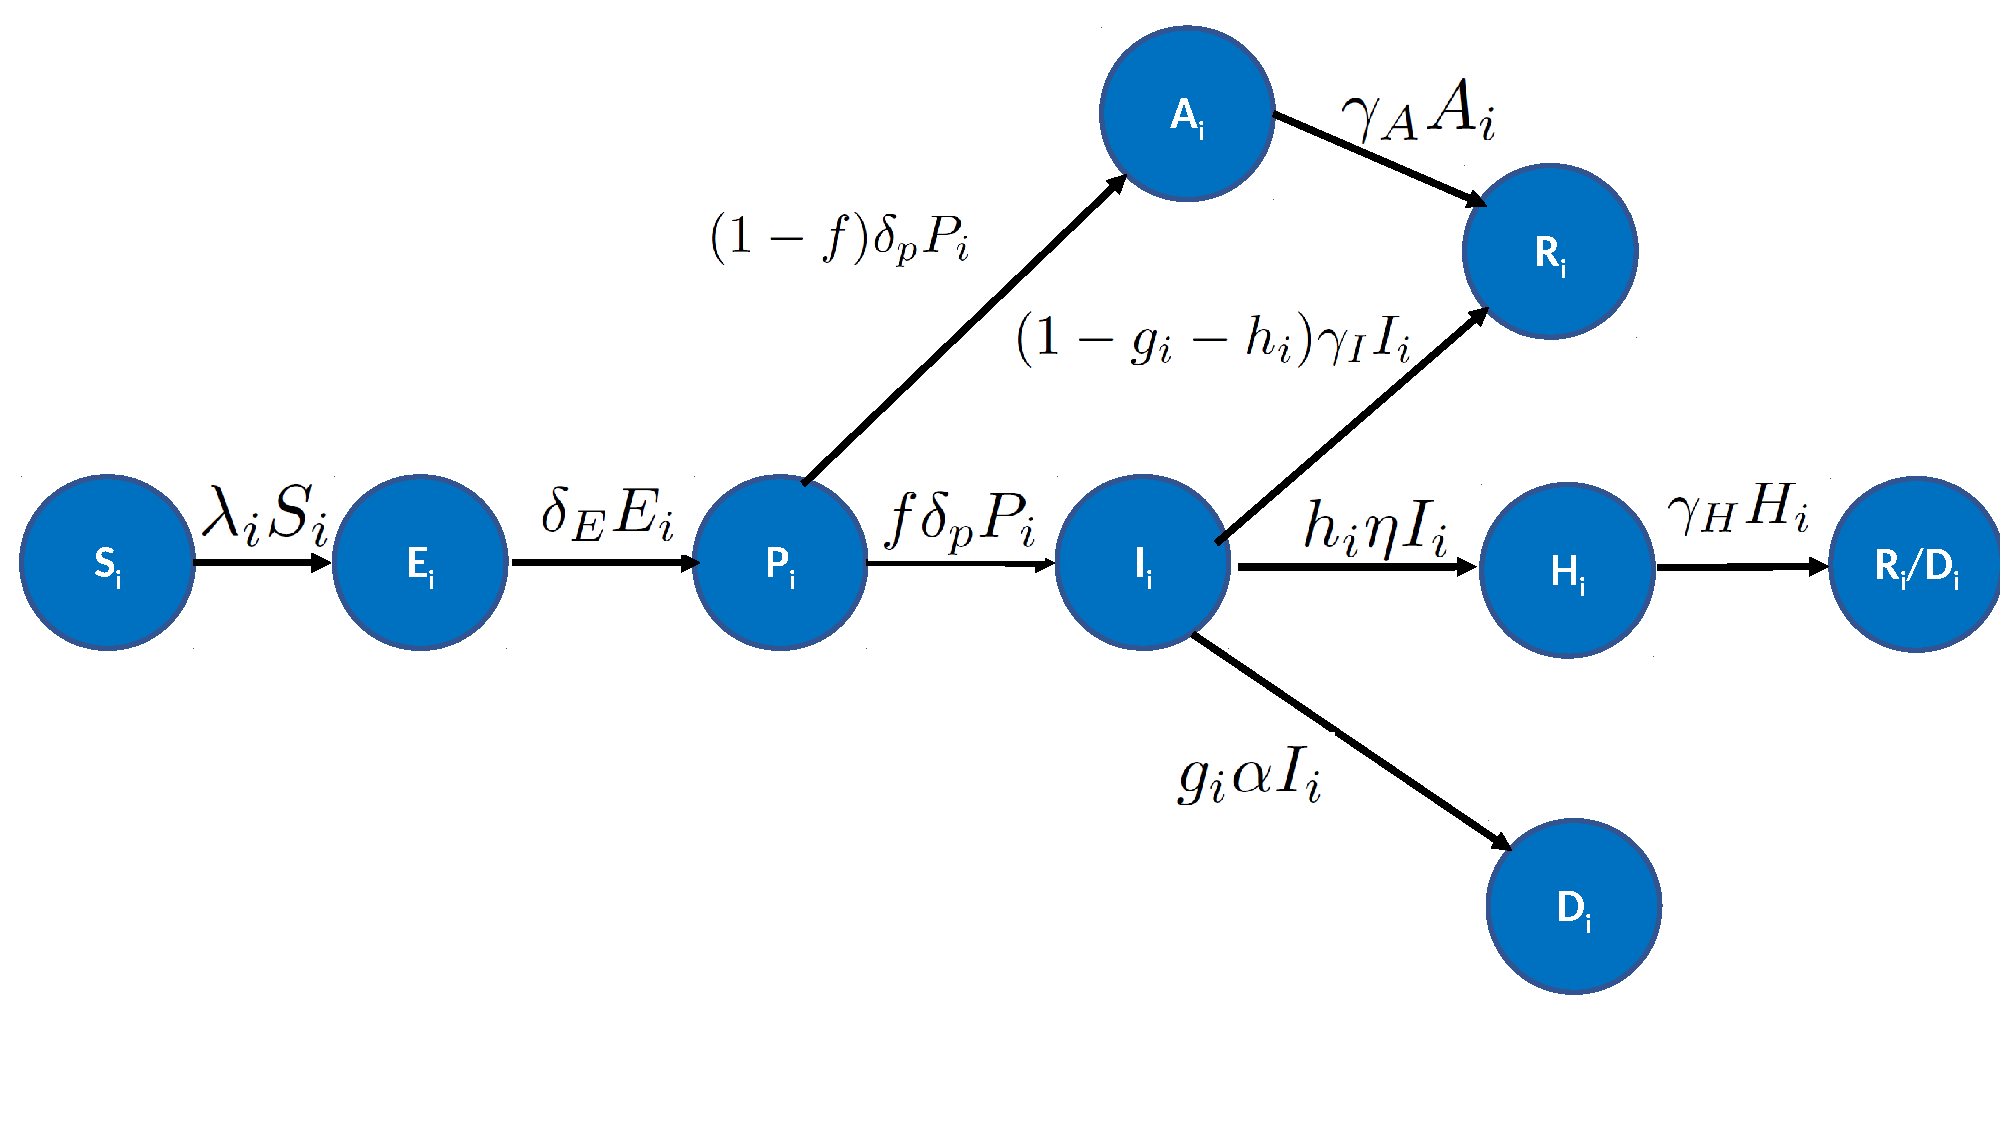
\includegraphics[width=.95\linewidth]{Model_graph_APG}
    \end{figure}
\end{frame}

\begin{frame}{Strategy 1: Self-distancing}

    \begin{columns}[t]
        \begin{column}{.5\textwidth}
        \begin{block}{Description}
        \begin{itemize}
            \item Reduction of number of contacts between individuals
            \item 
        \end{itemize}
        \end{block}
        \end{column}
        \begin{column}{.5\textwidth}
            \begin{block}{Key-points}
            \begin{itemize}
                \item Remark 1
                \item Remark 2
                \item Very simple measure.
                \item Relies on the individuals following the advice.
            \end{itemize}
            \end{block}
        \end{column}
    \end{columns}

\end{frame}

\begin{frame}{Strategy 1: Self-distancing}

Insert figure here.

\end{frame}

\begin{frame}{Strategy 2: Shielding}

    \begin{columns}[t]
        \begin{column}{.5\textwidth}
        \begin{block}{Description}
        \begin{itemize}
            \item Shield the most vulnerable population in a separate area of the camps.
            \item Vulnerable population: elderly and people with comorbidities.
            \item A low number of carers and family members are also shielded.
            
        \end{itemize}
        \end{block}
        \end{column}
        \begin{column}{.5\textwidth}
            \begin{block}{Key-points}
            \begin{itemize}
                \item Remark 1
                \item Remark 2
                \item Advantage
                \item Caveat
            \end{itemize}
            \end{block}
        \end{column}
    \end{columns}

\end{frame}

\begin{frame}{Strategy 2: Shielding}

Insert figure here.

\end{frame}

\begin{frame}{Strategy 3: Isolation}

    \begin{columns}[t]
        \begin{column}{.5\textwidth}
        \begin{block}{Description}
        \begin{itemize}
            \item Isolation of infected individuals
            \item cha
        \end{itemize}
        \end{block}
        \end{column}
        \begin{column}{.5\textwidth}
            \begin{block}{Key-points}
            \begin{itemize}
                \item Remark 1
                \item Remark 2
                \item We are assuming a quick response
                \item We are assuming perfect isolation
            \end{itemize}
            \end{block}
        \end{column}
    \end{columns}

\end{frame}

\begin{frame}{Strategy 3: Isolation}

Insert figure here.

\end{frame}


\begin{frame}{Combination of strategies}

\end{frame}

\begin{frame}{Conclusion}

\end{frame}



\end{document}
